\chapter{Standardization}

\section{Problem Statement}
The standardization process is a process to convert the instrumental values to physical values. In CCD, what is being read is the potential ($ \propto $ number of electrons $ \propto $ flux). But what does a CCD pixel value mean? $ 1 $ ADU can mean $ \SI{1}{Jy} $ at one CCD but at different one it can mean $ \SI{5}{Jy} $ because it is designed to be insensitive to photons for some reason. Thus, what astronomers do is

\begin{enumerate}
\item Make a list of objects which have known flux (e.g., star A has spectrum of blahblah, and it has $ \mathrm{V}_0 $ magnitude or flux $ I_0 $ in the V-band). These stars are called \textbf{standard stars}.
\item Observe the target and the standard stars simultaneously. 
\end{enumerate}
Now the power of CCD comes in: It's highly linear, i.e., the pixel counts of $ N $ (of the target of interest) and $ N_0 $ are very much proportional to the original flux, $ I $ and $ I_0 $. Thus, you can use Pogson's formula, because what it requires is only the ratio of flux: 
\begin{equation}\label{eq: Pogson}
  \mathrm{V} - \mathrm{V}_0 = -2.5 \lg \frac{I}{I_0} =  -2.5 \lg \frac{N}{N_0} ~.
\end{equation}

\begin{ex}[Simplest Standardization]
If the aperture photometry gave pixel count of $ 1000 $ for a standard star of $ \mathrm{V}_0 = \m{10.00} $ and the object had pixel count of $ 500 $, the above formula will give $ \mathrm{V} = \m{10.75} $. 
\end{ex}

In practice\footnote{From here, I extensively refered to Ch. 6 of ``A Practical Guide to Lightcurve Photometry and Analysis'' by Brian D. Warner, 2e.}, it is very difficult to use these formula. Because
\begin{enumerate}
\item The atmosphre exists. The magnitude we observe on ground is different from the one we would have observed outside of the atmosphere (space). This gives the $ k' $ and $ k'' $ terms in \cref{eq: std} below.
\item The CCD is not perfect. For example, if it is more sensitive to redder wavelength, making red stars brighter than they should be. This gives the $ k $ term in \cref{eq: std} below.
\end{enumerate}
After these are considered, we can obtain the following second-order approximation of the standard magnitude of an object seen on CCD:
\begin{equation}\label{eq: std}
  M_f = m_f - k_f' X - k_f''XC + z_f + k_f C \equiv m_{0f} + z_f + k_f C ~,
\end{equation}
where
\begin{equation}
  m_{f} = m_{0f} + k_f'X + k_f'' XC
\end{equation}
and
\begin{itemize}
\item $ f $: The filter (V, B, g', etc).
\item $ X $: airmass (secant of zenith angle).
\item $ M_f $: The standard apparent magnitude (or the true apparent magnitude) at filter $ f $. Also called the extra-atmospheric magnitude.
\item $ m_f $: The instrumental magnitude, i.e., $ -2.5 \lg N $.
\item $ m_{0f} $: The $ m_f $ value we would have obtained if we were in space ($ X = 0 $).
\item $ C $: The true color index, e.g., $ \mathrm{B} - \mathrm{V} $ or $ \mathrm{r'} - \mathrm{i'} $.
\item $ k_f' $: The first order extinction coefficient at filter $ f $.
\item $ k_f'' $: The second order extinction coefficient at filter $ f $.
\item $ z_f $: The zero point at filter $ f $.
\item $ k_f $: The system transform coefficient.
\end{itemize}
I will explain the terms related to $ m_{0f} $ and then the other terms. Note that lower- and upper-cased letters are used for the instrumental and true magnitudes, respectively (e.g., v and V, b and B, $ m_\mathrm{g'} $ and $ M_\mathrm{g'} $, etc).

%The example I showed with \cref{eq: Pogson} is the case when $ k_f = k_f' = k_f'' = 0 $, or equivalently $ k_f = 0 $ and $ X = 0 $. In such a case, the true apparent magnitude is $ \mathrm{V} = \mathrm{v} + z_\mathrm{V} = -2.5 \lg N + z_\mathrm{V} $ where $ \mathrm{v} $ is the instrumental magnitude and $ z_\mathrm{V} $ is just a constant\footnote{}. Same goes true for the standard star, so $ \mathrm{V}_0 = \mathrm{v}_0 + z_\mathrm{V} = -2.5 \lg N_0 + Z_\mathrm{V} $. Then \cref{eq: Pogson} makes sense and $ \mathrm{V}- \mathrm{V}_0 = \mathrm{v} - \mathrm{v}_0 $. If the coefficients are non-zero, you can see that 

From \cref{eq: std}\footnote{$ z_{f} $ must be a constant unless the device is affected by external disturbance in our simple model dealt in this chapter. In reality it is true that this zero point fluctuate at each exposure, and that is because of the imperfect readout process of CCD electronics. $ \Delta z_\mathrm{V} \approx 0 $ is assumed in this chapter.}:
\begin{equation}
  \mathrm{V} - \mathrm{V}_0 
    = (\mathrm{v} - \mathrm{v}_0)
    + k_\mathrm{V}'(X - X_0)
    + k_\mathrm{V}''(X C - X_0 C_0)
    + k_\mathrm{V}(C - C_0)
    + \Delta z_\mathrm{V}
    \neq \mathrm{v} - \mathrm{v}_0 ~.
\end{equation}
So the calculation given in the example is true only if the airmass of the object and standard star are identical AND the true color indices of them are identical, we cannot simply equate the right hand side of \cref{eq: Pogson}, which is $ \mathrm{v} - \mathrm{v}_0 $, to the left hand side. In space, $ X = 0 $ and $ \Delta z \approx 0 $, so only the $ k_f $ term remains. This is why space observation is powerful.

\section{Atmospheric Extinction}
The atmospheric extinction is dependent on the wavelength as in \cref{fig:air-ext-and-filter}. The extinction is severe at smaller wavelength, and that is why the sun look redder when it rises or sets (i.e., when airmass is larger). 

\begin{figure}[ht!]
\centering
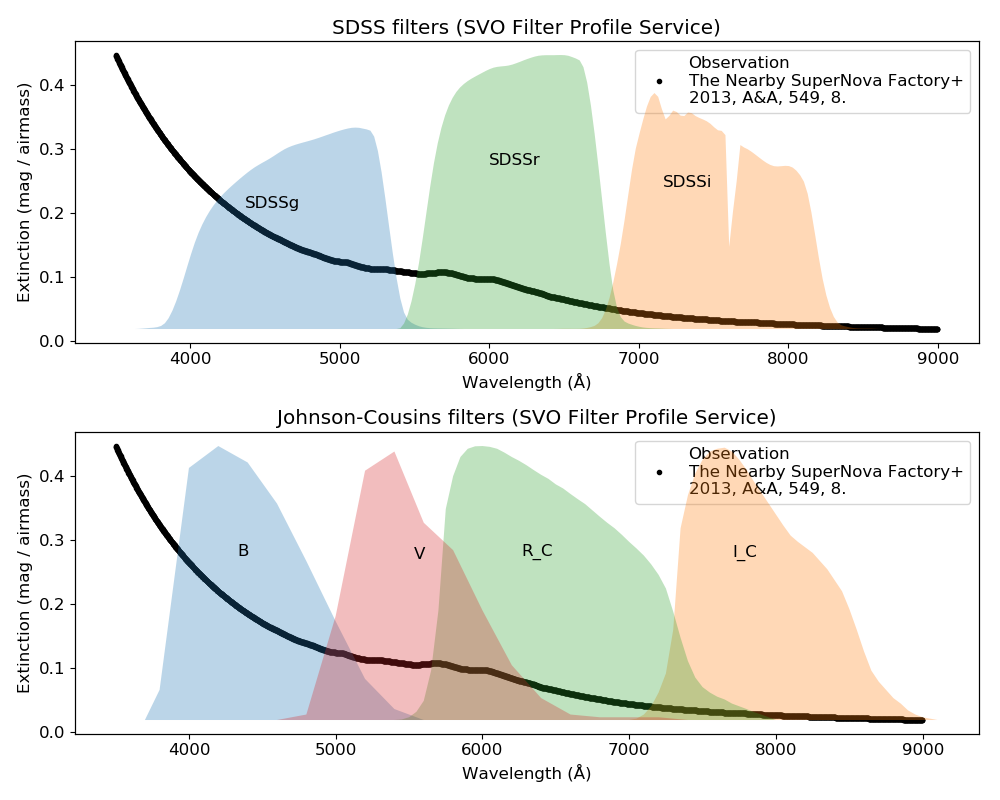
\includegraphics[width=0.9\linewidth]{figs/air-ext-and-filter}
\caption{The atmospheric extinction as a function of wavelength at Mauna Kea, \textit{based on some 4285 standard star spectra obtained on 478 nights spread over a period of 7 years obtained by the Nearby SuperNova Factory using the SuperNova Integral Field Spectrograph.} (excerpt from The Nearby SuperNova Factory+ 2013, A\&A, 549, 8). The SDSS and Johnson-Cousins filters' filter profiles are overplotted.}
\label{fig:air-ext-and-filter}
\end{figure}

Consider an object with spectrum $ S_0(\lambda) $ is at an airmass of $ X $ and underwent atmospheric extinction described by optical depth of $ \tau(\lambda) $. The magnitude at filter with profile $ f(\lambda) $ (say the filter has non-zero profile at $ \lambda \in (\lambda_1, \lambda_2) $) will have the following Pogson's relation:
\begin{equation}
  m_f - m_{0f}
    = -2.5 \lg
      \qty( \frac{\int_{\lambda_1}^{\lambda_2} S_0(\lambda) f(\lambda) e^{-\tau(\lambda) X} d\lambda}
      {\int_{\lambda_1}^{\lambda_2} S_0(\lambda) f(\lambda) d\lambda} ) ~.
\end{equation}
Here $ e^{-\tau(\lambda) X} $ is actually an approximation of $ e^{\int -\tau(\lambda) dX} $. Using Taylor expansions, $ e^{-\tau(\lambda) X} \approx 1 - \tau(\lambda) X $ and $ \lg (1 - A) \approx - A $, 
\begin{equation}
\begin{aligned}
    m_f - m_{0f} 
    &\approx -2.5 \lg 
      \qty( 1 - \frac{\int_{\lambda_1}^{\lambda_2} S_0(\lambda) f(\lambda) \tau(\lambda) d\lambda}
        {\int_{\lambda_1}^{\lambda_2} S_0(\lambda) f(\lambda) d\lambda} X ) 
    \approx 2.5 \frac{\int_{\lambda_1}^{\lambda_2} S_0(\lambda) f(\lambda) \tau(\lambda) d\lambda}
            {\int_{\lambda_1}^{\lambda_2} S_0(\lambda) f(\lambda) d\lambda} X ~.
\end{aligned}  
\end{equation}
Remembering $ I = I_0 e^{-\tau X} $, so $ \Delta m = -2.5 \lg (I / I_0) = 1.086 \tau X $, the y-axis of \cref{fig:air-ext-and-filter} is $ \sim 1.1 \tau $. Therefore, the approximation above is reasonable since $ \tau X \ll 1 $ for optical. (although this may break down in some cases like short wavelength high airmass observation, but the error due to this approximation may not be severe). 

Now we want to further assume that, $ \tau(\lambda) \approx c_1 + c_2 \lambda $ within the wavelength range of $ (\lambda_1, \lambda_2) $. This is similar to approximating the black markers in \cref{fig:air-ext-and-filter} within each filter as a line because its y-axis is nothing but $ 1.1 \tau $. Then
\begin{equation}
  m_f - m_{0f} 
    \approx 2.5 
    \qty (c_1 + c_2\frac{\int_{\lambda_1}^{\lambda_2} S_0(\lambda) f(\lambda) \lambda d\lambda}
      {\int_{\lambda_1}^{\lambda_2} S_0(\lambda) f(\lambda) d\lambda} ) X ~.
\end{equation}
If the filter is fixed (e.g., V-band or SDSS g filter, etc), the only unknown thing in the second term in the parenthesis is $ S_0(\lambda) $, i.e., the spectral shape. If it is a black body spectrum, it is true that the spectral shape has a one-to-one relationship with the color index\footnote{This is not strictly true. For example, at temperatures between $ T = \SI{15000}{K} $ and $ \SI{40000}{K} $, the color indices are $ \mathrm{B - V} = -0.20 $ and $ -0.30 $ which are almost indistinguishable. Furthermore, color index does not uniquely determine the temperature (e.g., $ \mathrm{B-V} $ is nearly the same for any object between 30,000 and 35,000 K). For your information, $ \mathrm{B-V} = 0.0 $ for 10,000 K black body, and the $ \mathrm{B-V} $ color is very useful to determine the temperature for $ T \lesssim \SI{10000}{K} $.}.
Even if it is not a perfect black body, it is reasonable to assume the spectral shape, $ S_0(\lambda) $, and color index, $ C $, have \textit{nearly} one-to-one relationship. Thus, $ C $ is an indicator of $ S_0(\lambda) $, so the second term is approximately a function of $ C $. The final assumption we make here is that the second term is $ c_3 + c_4 C $ as the first-order approximation. Here $ c_3 $ and $ c_4 $ depends on the filter profile. Then the parenthesis of the equation above becomes $ c_5 + c_6 C $ where $ c_5 $ and $ c_6 $ depends on the filter profile: $ m_f - m_{0f} \approx 2.5 (c_5 + c_6 C) X \equiv k_f' X + k_f'' CX $. These are the origins of $ k_f' $ and $ k_f'' $ in \cref{eq: std}.

To illustrate the result, I used the SDSS filter system as shown in \cref{fig:air-ext-bbrad} and calculated how much magnitude extinction happens depending on the black body temperature:

\begin{table}[ht!]
\centering
  \begin{tabular}{c||ccc}
  Temperature  & $ m_\mathrm{g'} - m_\mathrm{0 g'} $ & $ m_\mathrm{r'} - m_\mathrm{0 r'} $ & $ m_\mathrm{i'} - m_\mathrm{0 i'} $ \\
  \hline
  $ \SI{3000}{K} $  & $ \m{0.142} $ & $ \m{0.081} $ & $ \m{0.034} $ \\
  $ \SI{6000}{K} $  & $ \m{0.158} $ & $ \m{0.084} $ & $ \m{0.035} $ \\
  $ \SI{20000}{K} $ & $ \m{0.171} $ & $ \m{0.087} $ & $ \m{0.036} $ \\
  \end{tabular}
\end{table}

\begin{figure}[ht!]
\centering
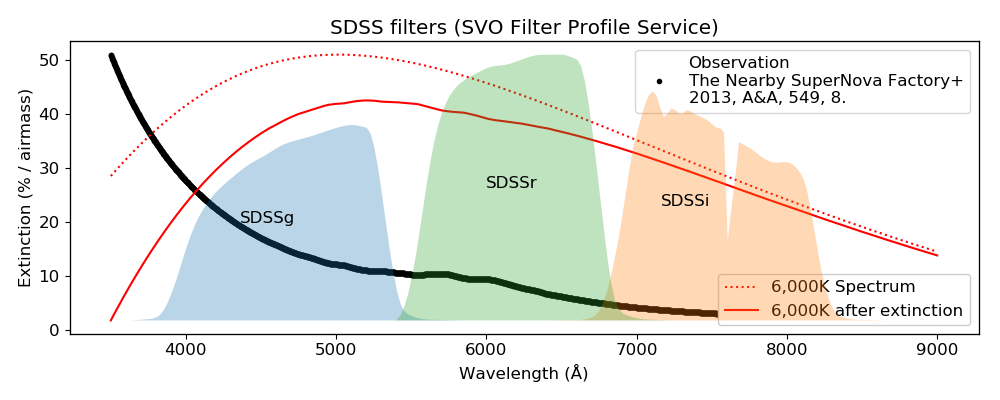
\includegraphics[width=0.9\linewidth]{figs/air-ext-bbrad}
\caption{A black body radiation spectrum ($ T = \SI{6000}{K} $) before and after the extinction at SDSS bands. Note that the y-axis is changed to \% per airmass (cf. \cref{fig:air-ext-and-filter}) by $ 10^{-0.4 \Delta m} $.}
\label{fig:air-ext-bbrad}
\end{figure}

As can be seen, the extinction is stronger for high temperature objects (lower color index), so we should have $ k_f'' < 0 $. The difference of extinction between the objects gets smaller as we look at longer wavelength.

These facts can be understood intuitively. The higher the temperature the spectrum will have more fraction of energe at shorter wavelength. Considering that the atmospheric extinction is stronger at shorter wavelength (see black markers in \cref{fig:air-ext-bbrad}), high termperature object will get more ``penalty'' when it comes into the atmosphere. That is why high temperature object is more strongly extincted. But as can be seen, the extinction gets nearly constant at wavelengths of r and i bands. Then this effect will get weaker and that is the reason for smaller discrepancy in $ \Delta m $ values at longer wavelength.



%Atmosphere diminishes the flux of the object. For an optical depth of $ \tau $, an object with initial flux $ I_0 $ will be observed as $ I = I_0 e^{-\tau} $ and its magnitude will be increased (because flux is decreased) by $ \Delta m = -2.5 \lg (I / I_0) = \frac{2.5}{\lg e} \tau = 1.086 \tau $. But $ \tau = \int n \sigma dl $ for the number density of particles $ n $, the extinction cross-section $ \sigma $, and traveling distance $ l $. The total traveling distance, $ L $, is $ L_0 / \cos z = L_0 X $ where $ X $ is the airmass. Thus, a simple approximation that $ \tau \propto L $ will result in $ \Delta m \propto X $. 

%The real story is more complicated: This extinction is of course wavelength-dependent (\cref{fig:air-ext-and-filter}). The black markers show the extinction magnitude per airmass. At zenith, $ X = 1 $ by definition, so this means that $ \Delta m \sim \m{0.2} $ at $ \lambda = \SI{4000}{\AA} $ but is $ \Delta m \ll \m{0.1} $ for $ \lambda = \SI{8000}{\AA} $. Therefore, the extinction is not simply proportional to $ X $, but the proportionality is a function of wavelength.

%\begin{thm}[Atmospheric Extinction: 1st Order]
%The extinction due to the atmosphere has the following 1st order term:
%\begin{equation*}
%  \Delta m(\lambda) = k'(\lambda) X ~,
%\end{equation*}
%where $ k'(\lambda) $ is the first-order extinction coefficient and is a function of wavelength $ \lambda $. In photometry, we are dealing with filters rather than each single wavelength, so normally we denote 
%\begin{equation}\label{eq: air-ext 1st ord}
%  \Delta m_f = k_f' X ~.
%\end{equation}
%\end{thm}
 

%Consider a black body spectrum is underwent this atmospheric extinction: \cref{fig:air-ext-bbrad}. The extinction is of course a function of wavelength. 

%In photometry, we are interested in the total number of photons \textit{after} multiplied with the filter profile: $ \int_{\lambda_1}^{\lambda_2} S(\lambda) f(\lambda) d\lambda $ where $ S(\lambda) $ is the spectrum and $ f(\lambda) $ is the filter profile. Thus, the magnitude change before and after the atmospheric extinction is, if the extinction is $ E(\lambda) $,
%\begin{equation}
%  \Delta m = 
%    -2.5 \lg \qty (\frac{\int_{\lambda_1}^{\lambda_2} E(\lambda) S(\lambda) f (\lambda) d\lambda}{\int_{\lambda_1}^{\lambda_2} S(\lambda) f(\lambda) d\lambda} )
%\end{equation} 
%Because it contains a ratio of the integration, it is not simple to calculate $ \Delta m $. From target to target, what changes is, except for the airmass (Note that $ E(\lambda) = e^{-\tau} \propto \sim e^X $), the $ S(\lambda) $. Thus, $ \Delta m = \Delta m (X, S) $. For a black body, this is a function of the temperature, and the temperature has (roughly) one-to-one counterpart of the color index. Thus, if the spectral shape is assumed as black body, we can write $ \Delta m = \Delta m (X, C) $ where $ C $ is the true color index. Even if it is not a black body, it is sufficient if the spectral shape and color index have \textit{nearly} one-to-one relationship. The extinction due to the spectral shape should also be proportional to the airmass to the first order approximation. Thus, as an approximation, we add a term proportion to $ CX $ to  \cref{eq: air-ext 1st ord}:

%\begin{thm}[Atmospheric Extinction: 2nd Order]
%The extinction due to the atmosphere is:
%\begin{equation}
%  \Delta m(\lambda) = k'(\lambda) X + k''(\lambda) C X ~,
%\end{equation}
%where $ k''(\lambda) $ is the second order atmospheric extinction coefficient.
%In photometry, we are dealing with filters rather than each single wavelength, so normally we denote 
%\begin{equation}\label{eq: air-ext 2nd ord}
%  \Delta m_f = k_f' X + k_f'' C X ~.
%\end{equation}
%\end{thm}


